%% ==============================
\chapter{How to use}
%% ==============================

\section{Getting Started}
If you are new to \LaTeX, please take a look at \url{https://de.overleaf.com/learn/latex/Learn_LaTeX_in_30_minutes}.

Initially you \textbf{should edit} the \texttt{my\_document\_info.tex} with important data regarding your work.

Adapt the second line of \texttt{main.tex} according to the language and type of your thesis. Regardless of language, both English and German abstracts should be written. You can also set the color of the H-KA logo (red or blue) there.

Add \textbf{content} in files in \texttt{content} folder.

Add \textbf{figures} in \texttt{figures} folder.

Add \textbf{bibliography} in the file \texttt{references.bib}.

As a useful aid in all scientific work the following book is recommended: \cite{deininger2005studien}.

Before your final submission, delete the line \texttt{\\include\{content/09-how-to-use\}} from \texttt{main.tex}.

\section{Inline lists}
My robot can:
\begin{enumerate*}[label=(\roman*)]
 \item forward and backward movements,
 \item sidewards movements,
 \item rotation along any curve in space,
 \item place of artificial forces along paths.
\end{enumerate*}

\begin{enumerate*}[label=(\arabic*),itemjoin={{; }}]
    \item the independently controllable wheels
    \item the rechargeable battery pack
    \item the Sick LMS100 laser range scanner
    \item the force-torque sensor
    \item the handlebar for controlling the robotic device
\end{enumerate*}

\url{https://ctan.math.illinois.edu/macros/latex/contrib/enumitem/enumitem.pdf}

\section{Todos}

Todo command can be used in multiple form and parameters set. You can set todos on the right side with commands:
{\small
\begin{verbatim}
\todo{Rewrite this section}
\todo[color=green]{Stuff}
\end{verbatim}
} which render as:
\todo{Rewrite this section}
\todo[color=green]{Stuff}



% \todo[due=2017-08-18]{Stuff}
% \todo[done]{Stuff}

You can also create inline todos with command:
{\small
\begin{verbatim}
\todo[inline]{Rewrite this section}
\todo[inline,color=green]{Rewrite this section}
\end{verbatim}
} which renders as:
\todo[inline]{Rewrite this section}
\todo[inline,color=green]{Rewrite this section}

One can also use command for figure placeholder with command:
{\small
\begin{verbatim}
 \missingfigure{Please add some figures}
\end{verbatim}
} which renders as:
\missingfigure{Please add some figures}


\section{Acronyms}
Please use \texttt{glossaries} package for this. See \href{https://en.wikibooks.org/wiki/LaTeX/Glossary}{\textit{documentation}}.

Example (Acronym):
{\small
\begin{spverbatim}
\newacronym{iras}{iRAS}{Institute for Applied Research - Robotics and Autonomous Systems}
\end{spverbatim}
} 
% \newacronym{iras}{iRAS}{Institute for Applied Research - Robotics and Autonomous Systems}
is used by
{\small
\begin{verbatim}
\gls{iras}
\end{verbatim}
}
% rendering as ``\gls{iras}'', on the first use and as ``\gls{iras}'' on every following use. For further feature see \href{https://en.wikibooks.org/wiki/LaTeX/Glossary}{\textit{documentation}}.


\section{SI Units}
Please use \texttt{siunitx} package for this. See:  \url{https://ctan.org/pkg/siunitx}

\section{Tables}
\begin{table}[H]
\caption{Tables have caption on top.}
\label{tab:table_caption}
\centering
\resizebox{\columnwidth}{!}{
 \begin{tabular}{| c | c | c | c |}
  \hline
  Object & Speed $[cm/s]$ & Inner LR $[cm]$ & Inner UR $[cm]$ \\ \hline \hline
  \multirow{3}{*}{\emph{Pitcher}} & real & $ n/a $ & $ 5.65 $ \\
   & $4.60$ & $3.71 \pm 0.67$ & $5.09 \pm 2.23$ \\
   & $10.64$ & $3.55 \pm 0.57$ & $6.14 \pm 0.69$ \\ \hline \hline
  \multirow{3}{*}{Cookie O} & real & $ 7.55 $ & $ 7.55 $ \\
   & $4.60$ & $6.98 \pm 0.27$ & $6.98 \pm 0.27$ \\
   & $10.64$ & $6.77 \pm 0.26$ & $6.77 \pm 0.26$ \\ \hline
 \end{tabular}
 }
\end{table}

Use \texttt{\textbackslash longtable} for tables over multiple pages. See \href{https://de.wikibooks.org/wiki/LaTeX-W%C3%B6rterbuch:_longtable_(Umgebung)}{documentation}.

\section{Figures}
\begin{figure}[H]
    \centering
    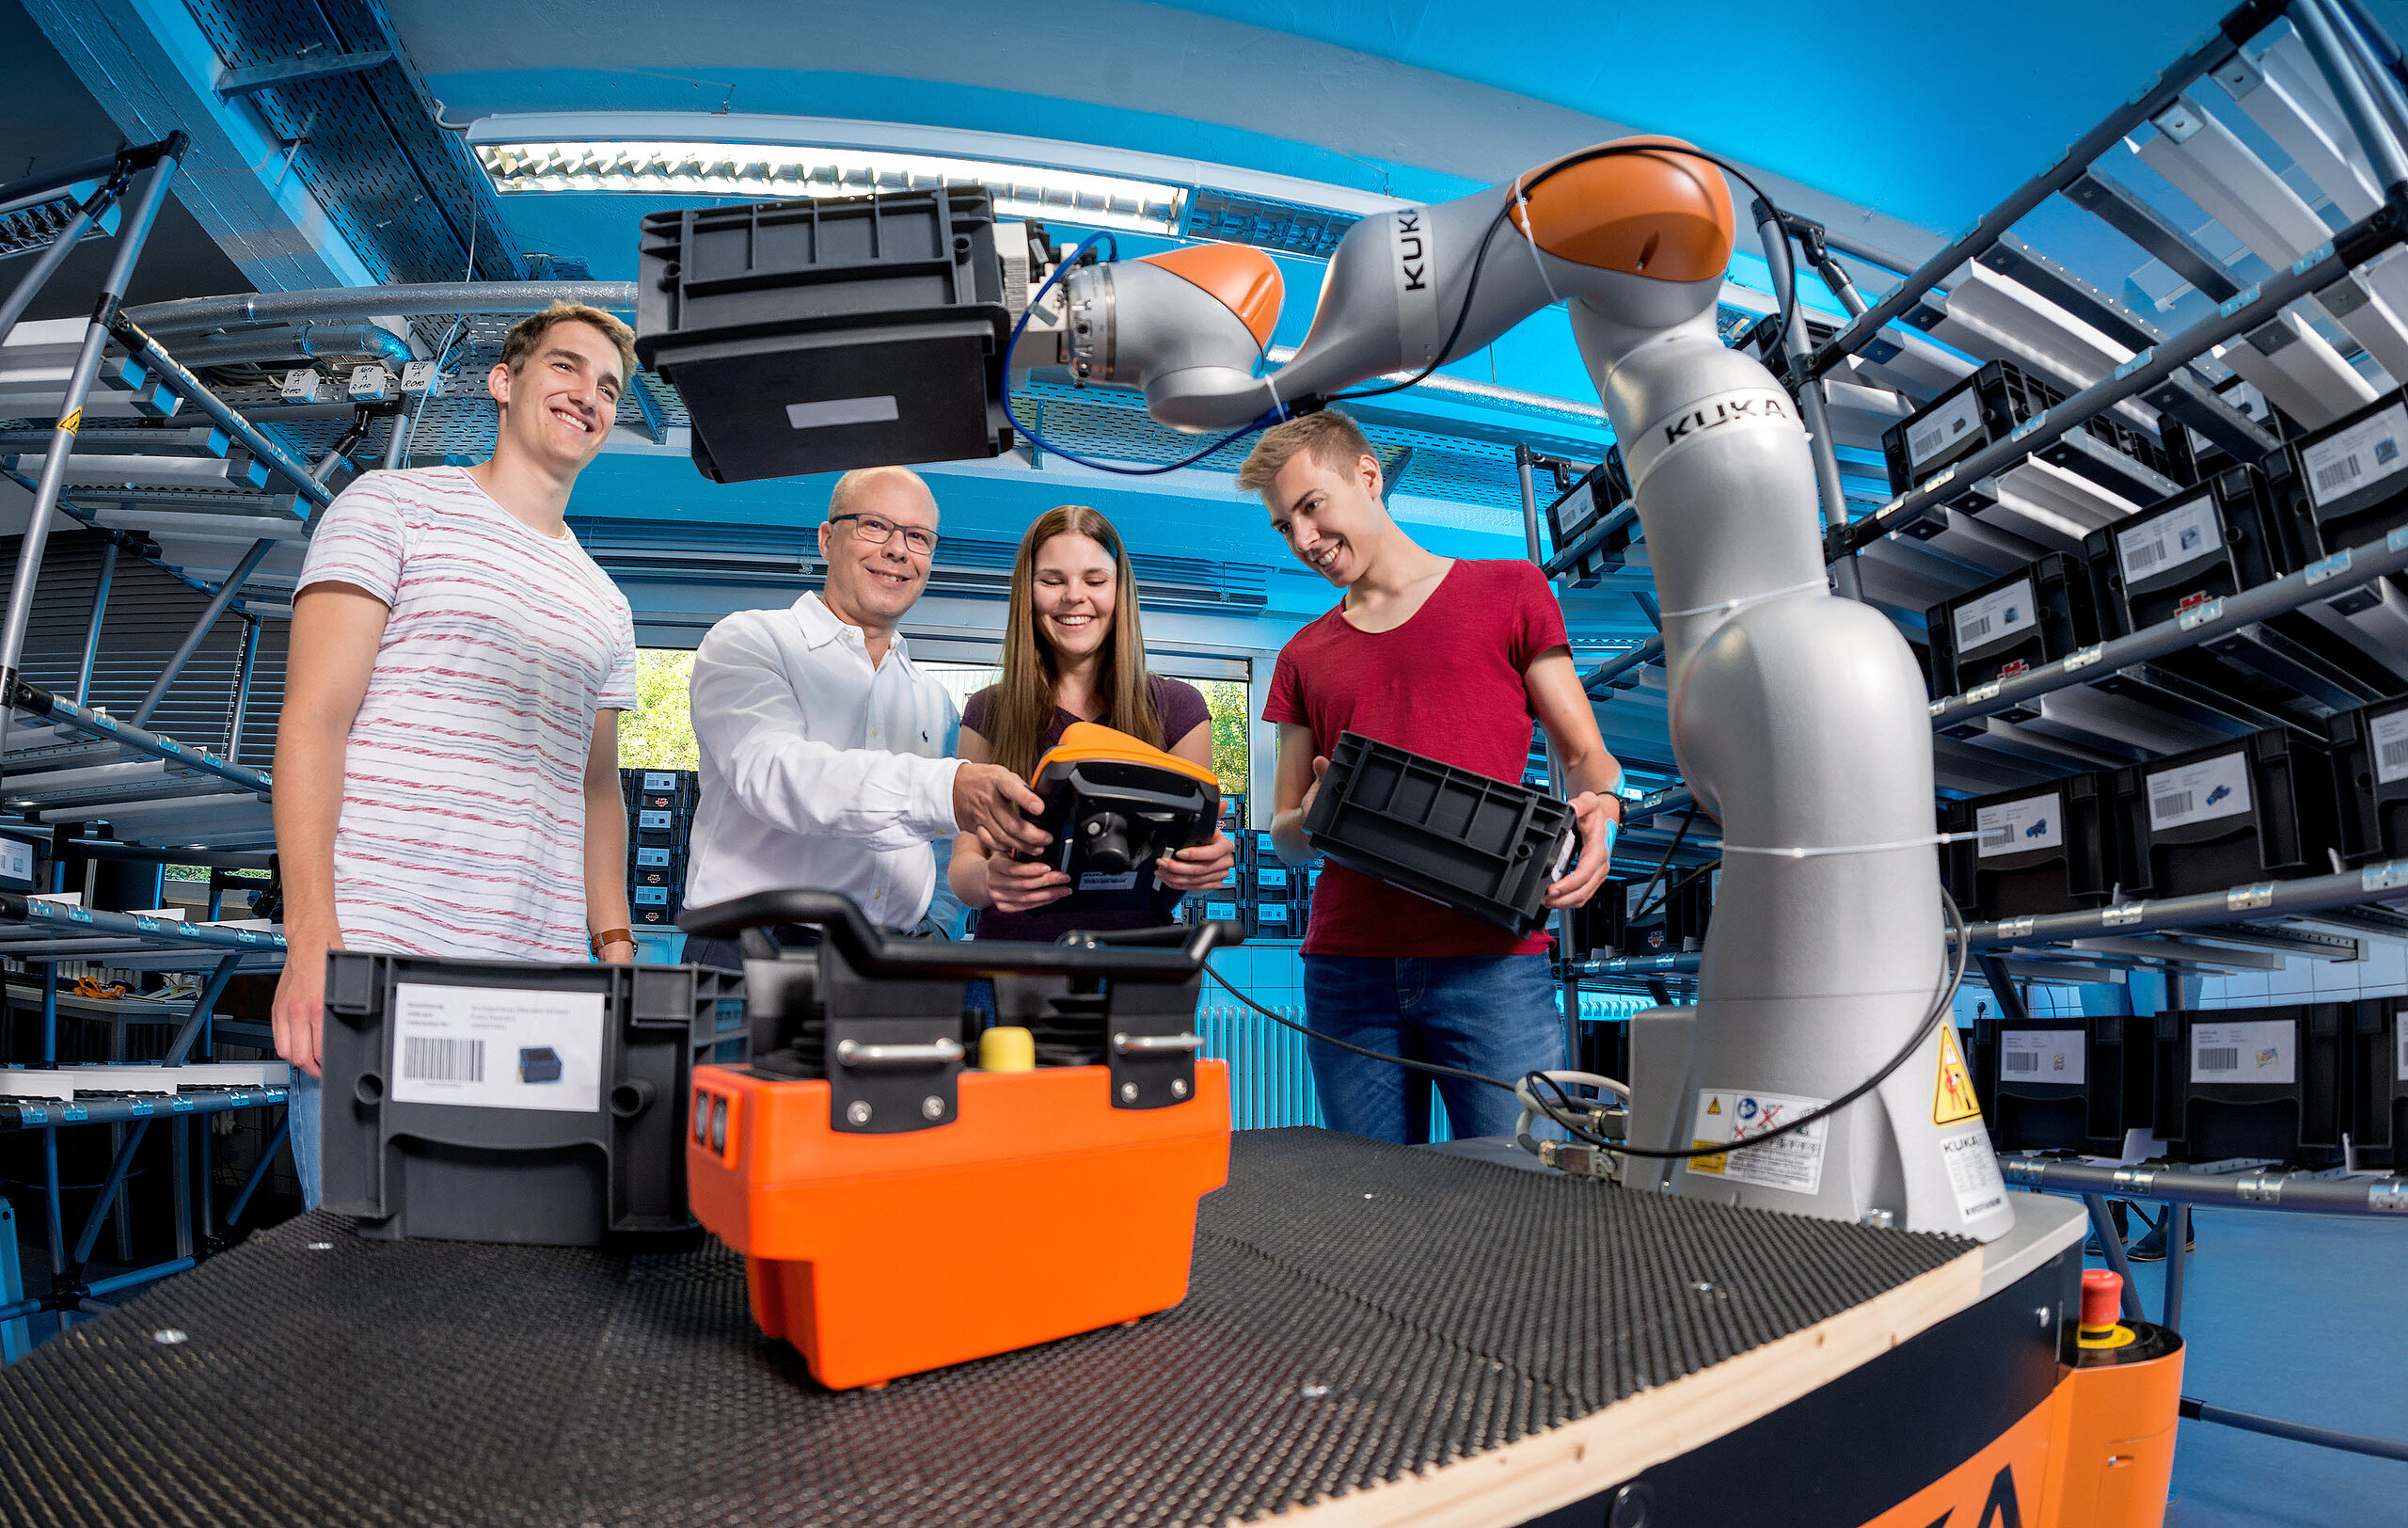
\includegraphics[width=\linewidth]{example_img}
    \caption{Figures have caption under. If you use figures from other work, do not forget to reference them \cite{deininger2005studien}.}
    \label{fig:figure_caption}
\end{figure}

\section{Subfigures}
%For more explanation see \href{https://en.wikibooks.org/wiki/LaTeX/Floats,_Figures_and_Captions#Subfloats}{Wikibooks}
\begin{figure}[H]
    \centering
    \begin{subfigure}[b]{0.3\textwidth}
        
\includegraphics[width=\textwidth]{logos/HKA_Bildmarke-v_CMYK}
        \caption{First logo}
        \label{fig:logo1}
    \end{subfigure}
    ~ %add desired spacing between images, e. g. ~, \quad, \qquad, \hfill etc.
      %(or a blank line to force the subfigure onto a new line)
    \begin{subfigure}[b]{0.3\textwidth}
        
\includegraphics[width=\textwidth]{logos/HKA_Bildmarke-v_CMYK}
        \caption{Second logo}
        \label{fig:logo2}
    \end{subfigure}
    ~ %add desired spacing between images, e. g. ~, \quad, \qquad, \hfill etc.
    %(or a blank line to force the subfigure onto a new line)
    \begin{subfigure}[b]{0.3\textwidth}
        
\includegraphics[width=\textwidth]{logos/HKA_Bildmarke-v_CMYK}
        \caption{Third logo}
        \label{fig:logo3}
    \end{subfigure}
    \caption{Pictures of Logos}\label{fig:logos}
\end{figure}


\section{Citation}

Use citations like this:
{\small
\begin{verbatim}
\cite{deininger2005studien}
\end{verbatim}
}
rendered as ``\cite{deininger2005studien}''.

\subsection{Multiple citations}
Use multiple citation like this:
{\small
\begin{verbatim}
\cite{deininger2005studien, deininger2005studien}
\end{verbatim}
}
rendered as ``\cite{deininger2005studien, deininger2005studien}''.

\section{Using Hyperlinks}
Please use the ability of PDF viewers to interpret hyperlinks\footnote{The example is from the template for the conference \href{http://www.roboticsconference.org/information/authorinfo/}{\textit{Robotic Science and Systems}}.}, specifically to allow each reference in the bibliography to be a
link to an online version of the reference.
As an example, if you were to cite ``Passive Dynamic Walking''
\cite{McGeer01041990}, the entry in the bibtex would read:

{\tiny
\begin{spverbatim}
@article{McGeer01041990,
  author = {McGeer, Tad},
  title = {\href{http://ijr.sagepub.com/content/9/2/62.abstract}{Passive Dynamic Walking}},
  volume = {9},
  number = {2},
  pages = {62-82},
  year = {1990},
  doi = {10.1177/027836499000900206},
  URL = {http://ijr.sagepub.com/content/9/2/62.abstract},
  eprint = {http://ijr.sagepub.com/content/9/2/62.full.pdf+html},
  journal = {The International Journal of Robotics Research}
}
\end{spverbatim}
}
\noindent
and the entry in the compiled PDF would look like:

\def\tmplabel#1{[#1]}

\begin{enumerate}
\item[\tmplabel{1}] Tad McGeer. \href{http://ijr.sagepub.com/content/9/2/62.abstract}{Passive Dynamic
Walking}. {\em The International Journal of Robotics Research}, 9(2):62--82,
1990.
\end{enumerate}
%
where the title of the article is a link that takes you to the article on IJRR's website.


Also use this for adding links into text as done in the \footnotemark[1]. For more information see documentation on \href{https://de.wikibooks.org/wiki/LaTeX-W%C3%B6rterbuch:_hyperref}{wikibooks}. The \texttt{hyperref} package is already configured for this document in \texttt{document\_setup.tex} file.


\section{Equations}
Use numbered equations:
\begin{equation} \label{equ:equ}
  m \cdot \ddot{x}(t) + d \cdot \dot{x}(t) = F(t)
\end{equation}

Reference equations, figures, tables or anything with a label by 

\begin{spverbatim}
\ref{label_name}
\end{spverbatim}
e.g. Equation \ref{equ:equ}

\section{Code or Algorithms}

\lstset{language=C++, caption={Pseudocode einer \textit{Sequence} mit \textit{N} Kindern}, label={lst:Pseudocode Sequence}}
\begin{lstlisting}
for i %\textbf{from}% 1 %\textbf{to}% %\textit{N}% do
    child_status = tick(child[i])
    if child_status == %\textit{Running}%
        return %\textit{Running}%
    if child_status == %\textit{Failure}%
        return %\textit{Failure}%
return %\textit{Success}%
\end{lstlisting}

\lstset{language=Python, caption={Python Skript zum Definieren eines Greifverhaltens}, label={lst:Python Greifverhalten}}
\begin{lstlisting}
def GraspObject(self):
    rospy.loginfo("Grasping an object from table...") # prepare for grasping
    myhandle = self.sss.Move("arm","pregrasp",False)
    self.sss.Move("sdh","cylopen")
    myhandle.wait()
    # grasp the object
    self.sss.Move("arm","grasp")
    self.sss.Move("sdh","cylclosed")
    # put object on tray
    myhandle = self.sss.Move("arm","grasp-to-tablet",False)
    self.sss.Move("tray","up")
    myhandle.wait()
    self.sss.Move("sdh","cylopen")
    # draw arm back to folded position
    myhandle = self.sss.Move("arm","tablet-to-folded",False)
    self.sss.Move("sdh","cylclosed")
    myhandle.wait()
\end{lstlisting}

